\chapter{Results}
\section*{Preliminary Results}
\label{sec:prelim}

To this point, I have been able to create scripts to import and assemble my multi-date images; to sample images and generate mean reference curves of the VI values for soy, corn, and wheat (Fig. \ref{fig:curves}; and to take said reference curves and generate an image for each crop, of which the pixel values are the RMSE after constrained minimization, and an image with the best fit for each pixel (Fig. \ref{fig:testing1}). For script development I am using MODIS 16-day EVI data from 2012. I have not completed the computation of the confidence scores of any given classification (a la fuzzy classification), but, for the sake of exploring this initial output, I used a threshold of .08 RMSE and classified the image according to the best fit. That is, for any pixels which had an RMSE of .08 or less for one or more of the crops tested, I used the best fit image values for those pixels as the values for classification (Fig. \ref{subfig:classification1}). I used the USDA CDL for 2012, resampled to 250 meter pixels with the majority value (Fig. \ref{subfig:CDL}), to check my classification. Building a confusion matrix for all of the pixels in the image resulted in Table \ref{table:acc}. As shown, the accuracies for each of the crops ranged between 60 percent and 70 percent, with an overall accuracy of 63 percent, though the kappa value is somewhat low at 0.44. Nonetheless, considering this is the unoptimized algorithm with an arbitrary threshold value, I believe my results suggest this classification method to have potential.

\begin{figure}
  \centering
  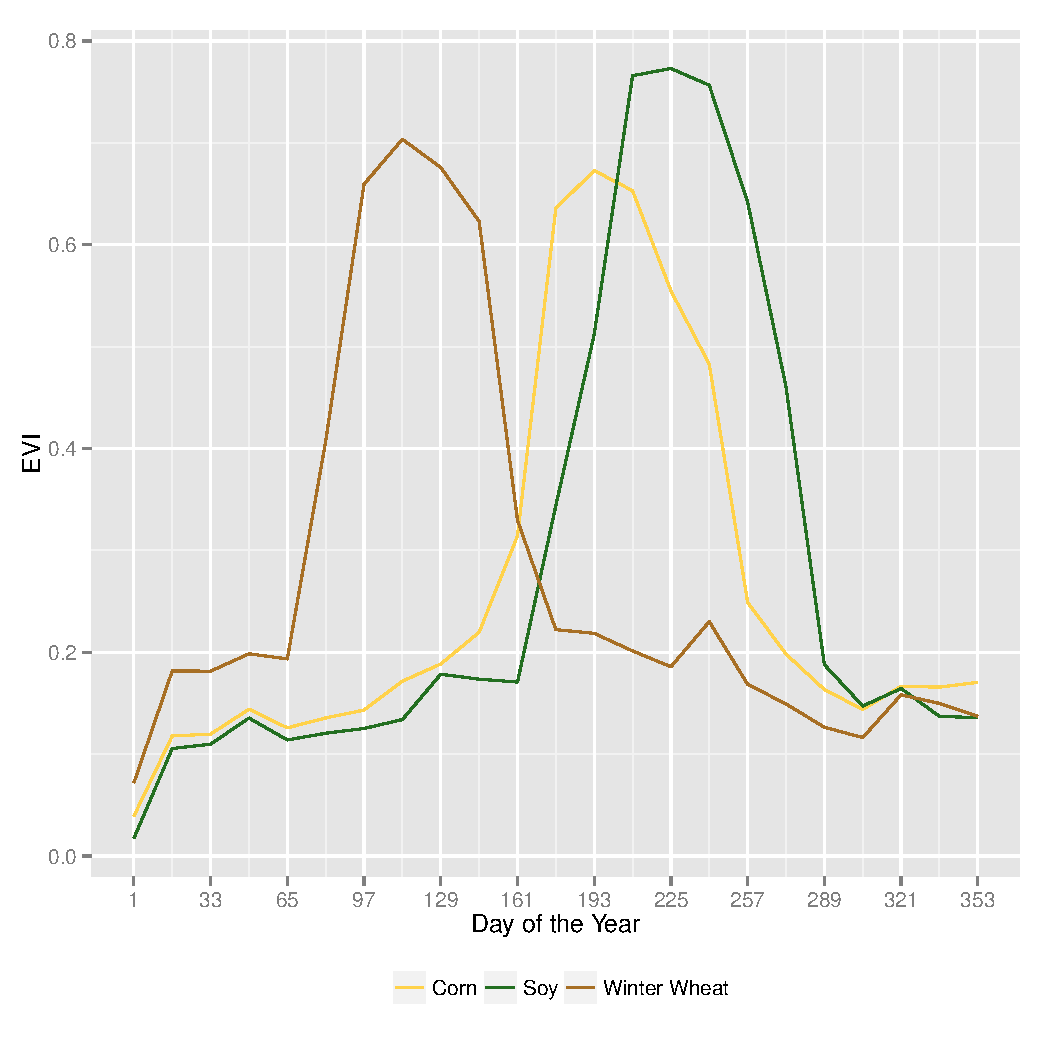
\includegraphics[width=\textwidth]{Graphics/cropCurves.pdf}
  \caption{Mean phenological curves found for corn, soy, and winter wheat. Each curve is generated from the mean EVI values of four pixels of the respective crop from an initial test area in 2012 Kansas data.}
  \label{fig:curves}
\end{figure}

\begin{figure}
  \centering
  \begin{subfigure}[b]{.45\textwidth}
    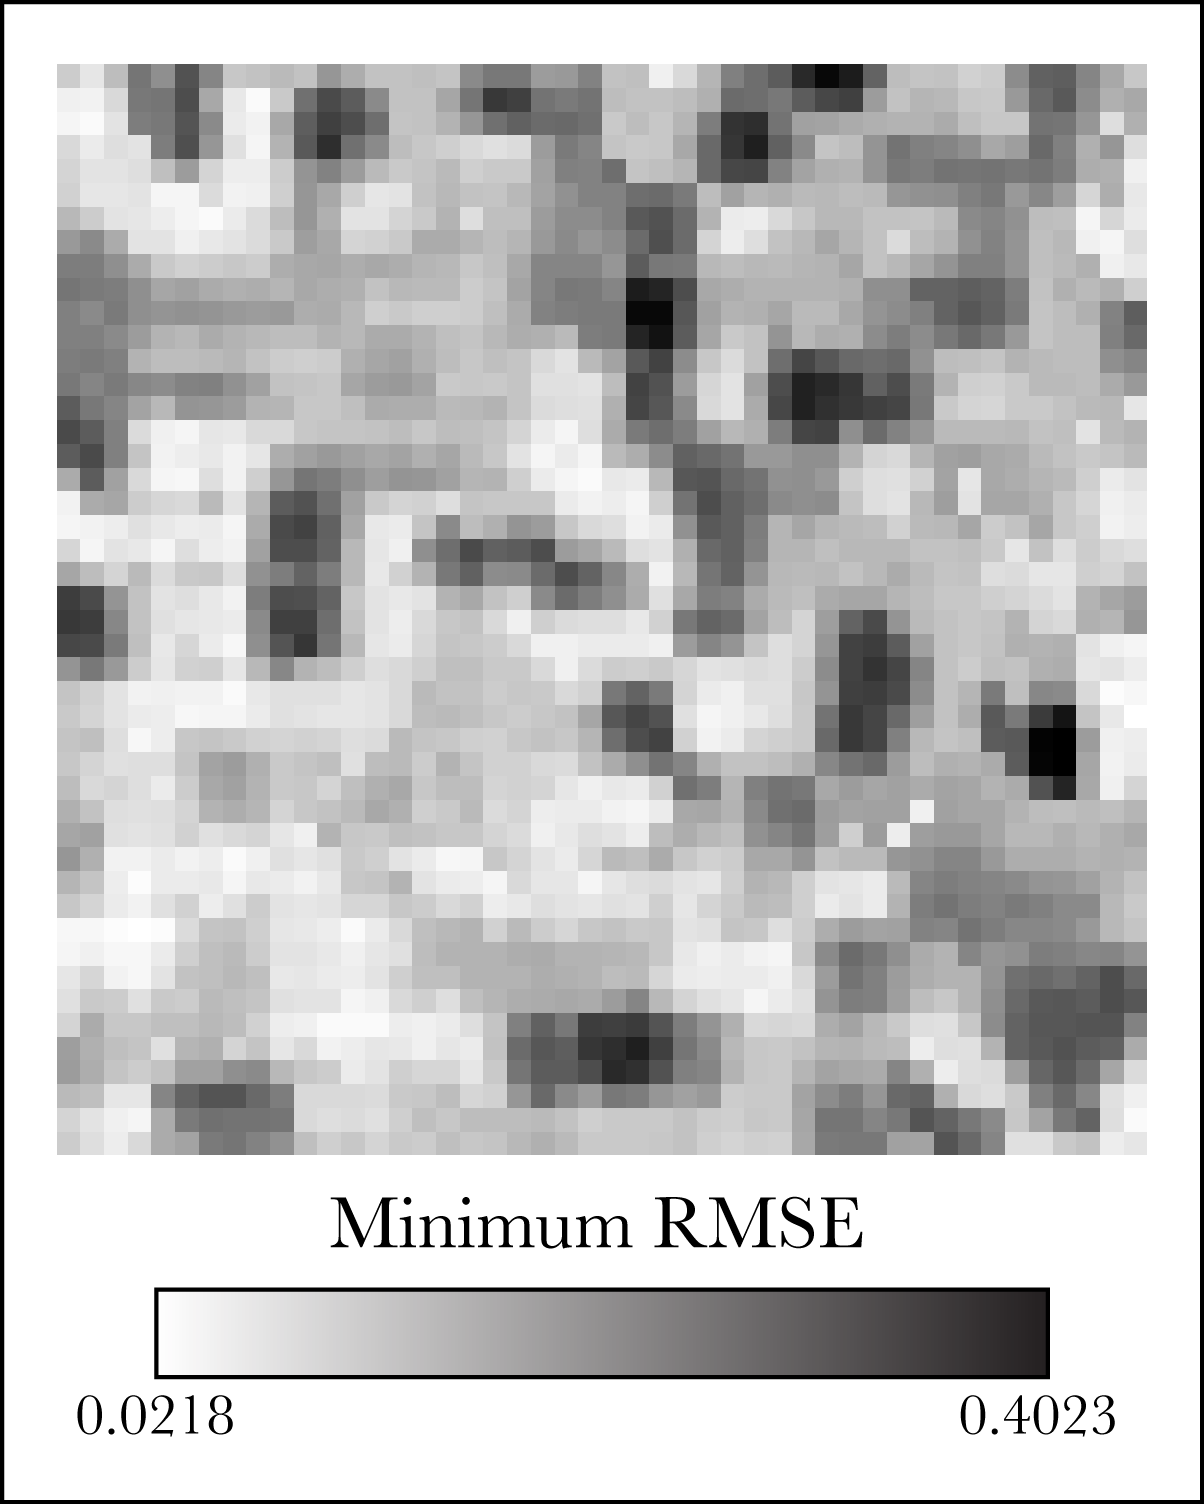
\includegraphics[width=\textwidth]{Graphics/corn1_edited.png}
    \caption{Fit of corn reference curve.}
    \label{subfig:corn1}
  \end{subfigure}
  \quad
  \begin{subfigure}[b]{.45\textwidth}
    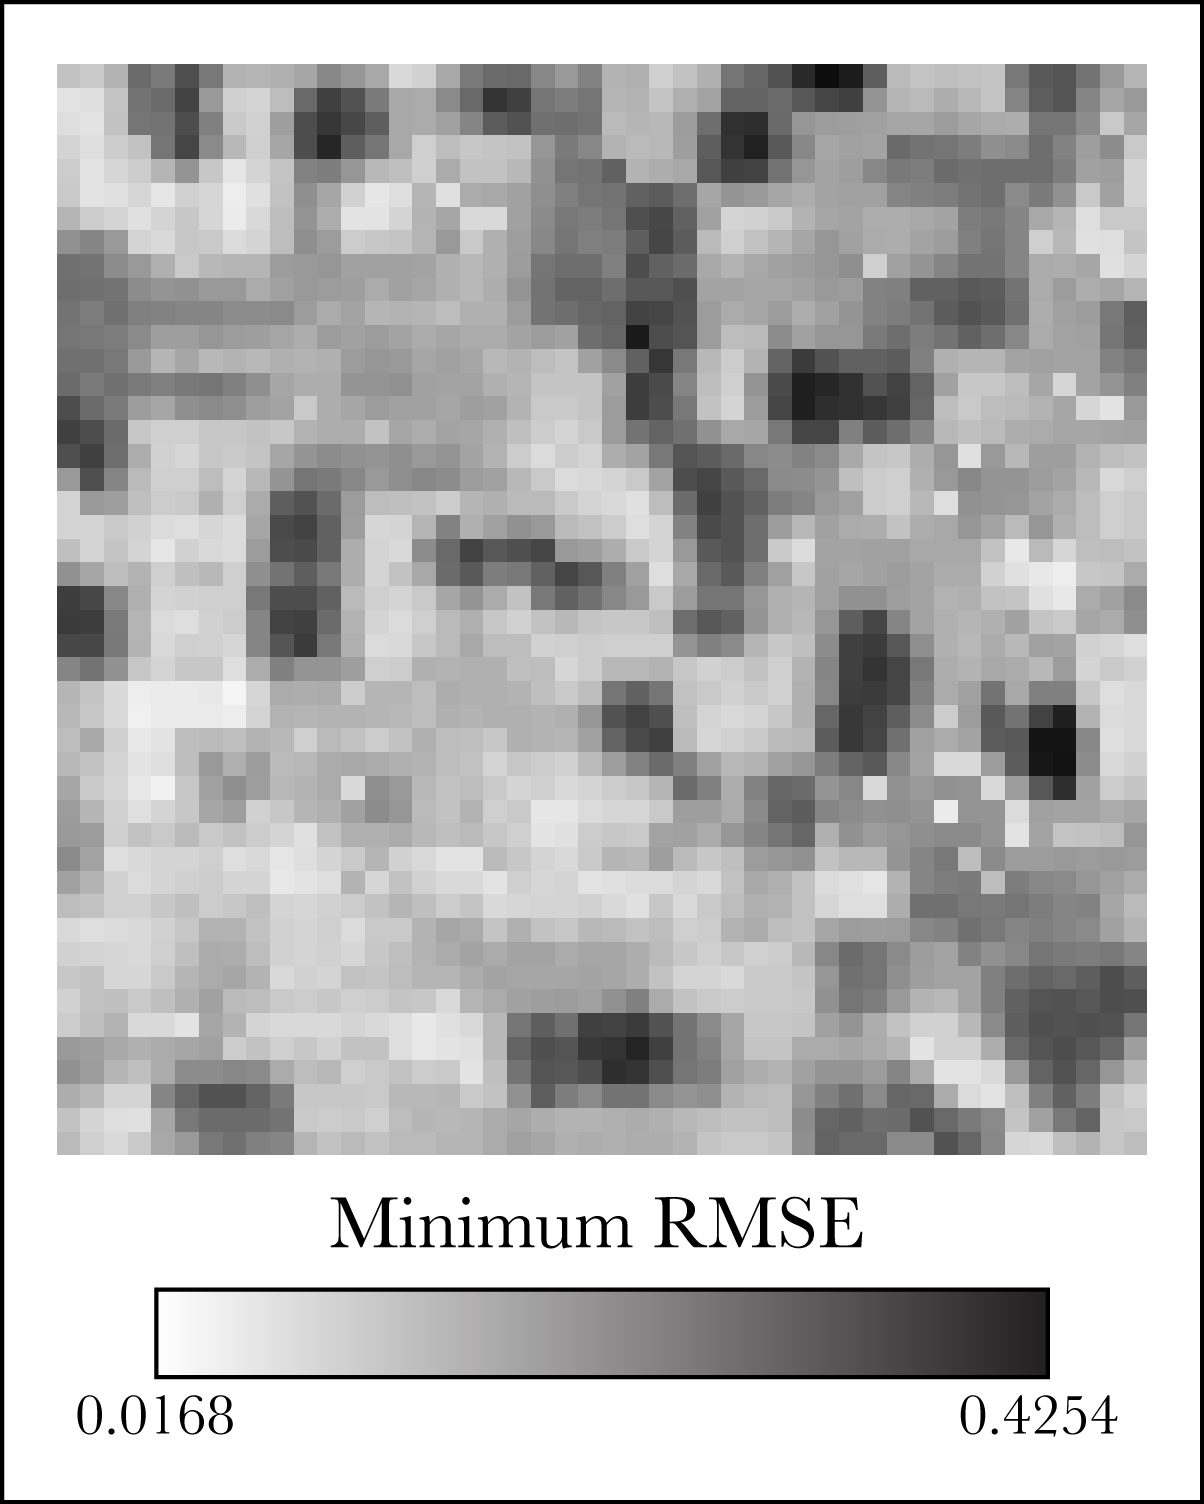
\includegraphics[width=\textwidth]{Graphics/soy1_edited.png}
    \caption{Fit of soy reference curve.}
    \label{subfig:soy1}
  \end{subfigure}
  \\
  \vspace{.25in}
  \begin{subfigure}[b]{.45\textwidth}
    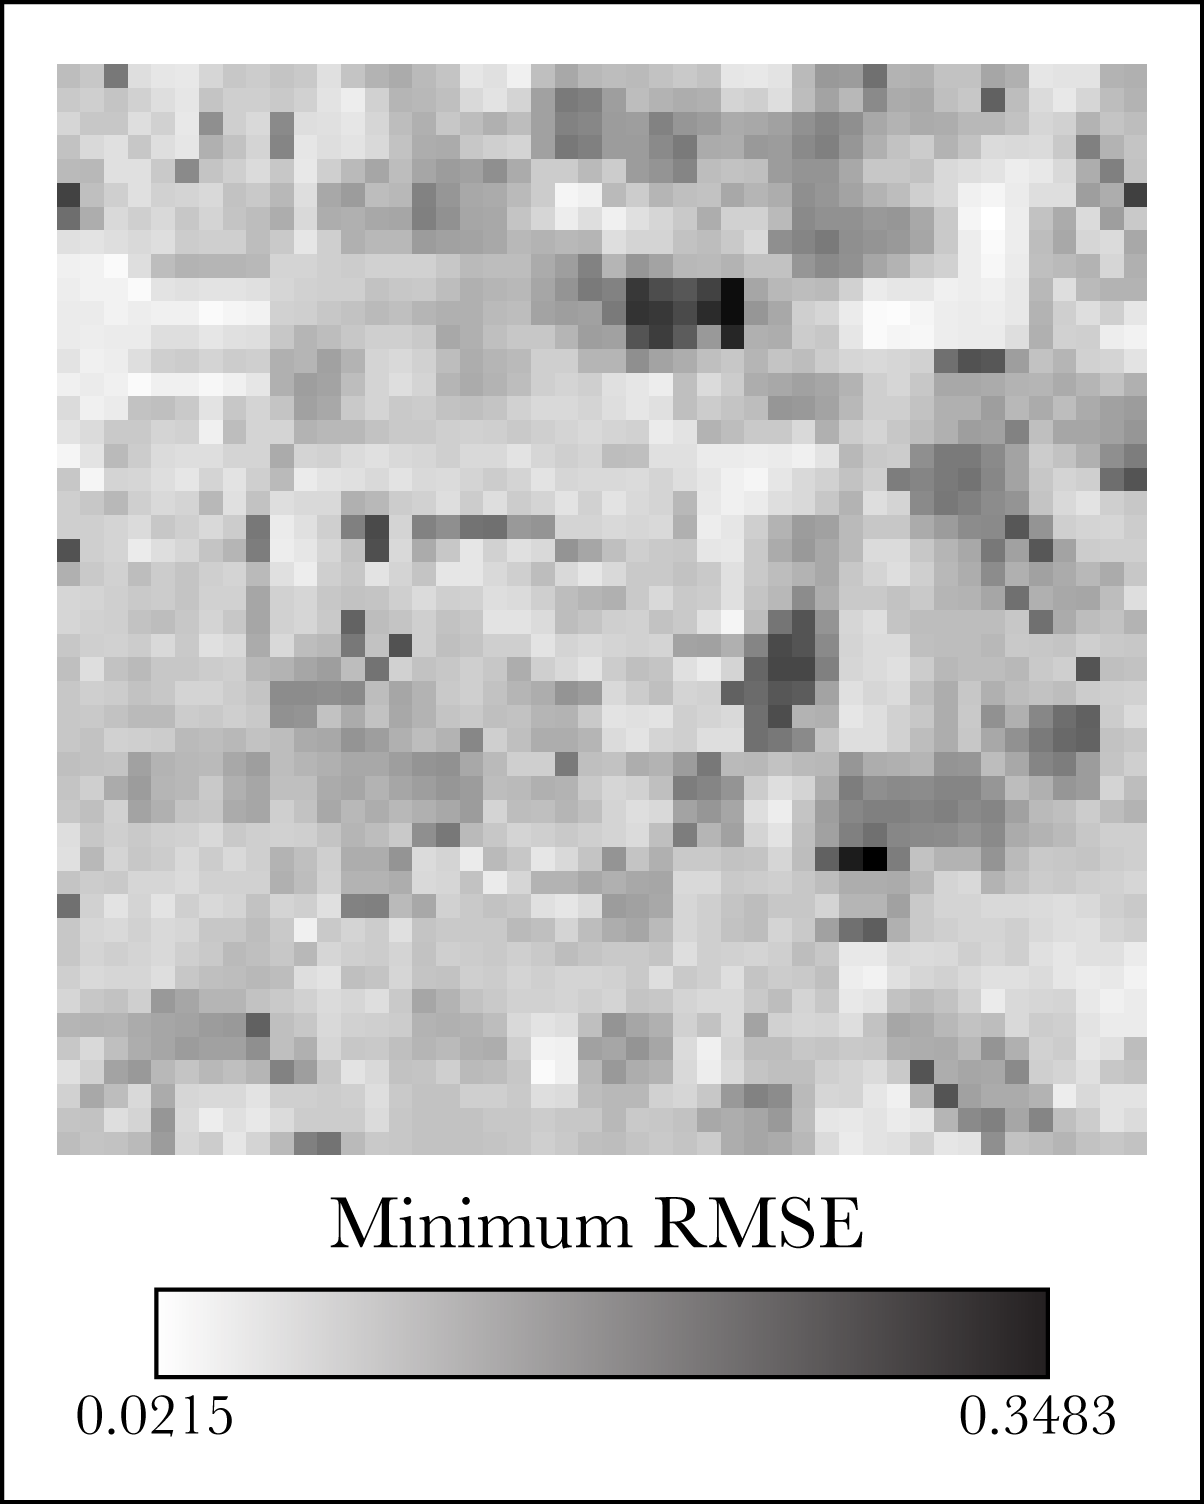
\includegraphics[width=\textwidth]{Graphics/wheat1_edited.png}
    \caption{Fit of wheat reference curve.}
    \label{subfig:wheat1}
  \end{subfigure}
  \quad
  \begin{subfigure}[b]{.45\textwidth}
    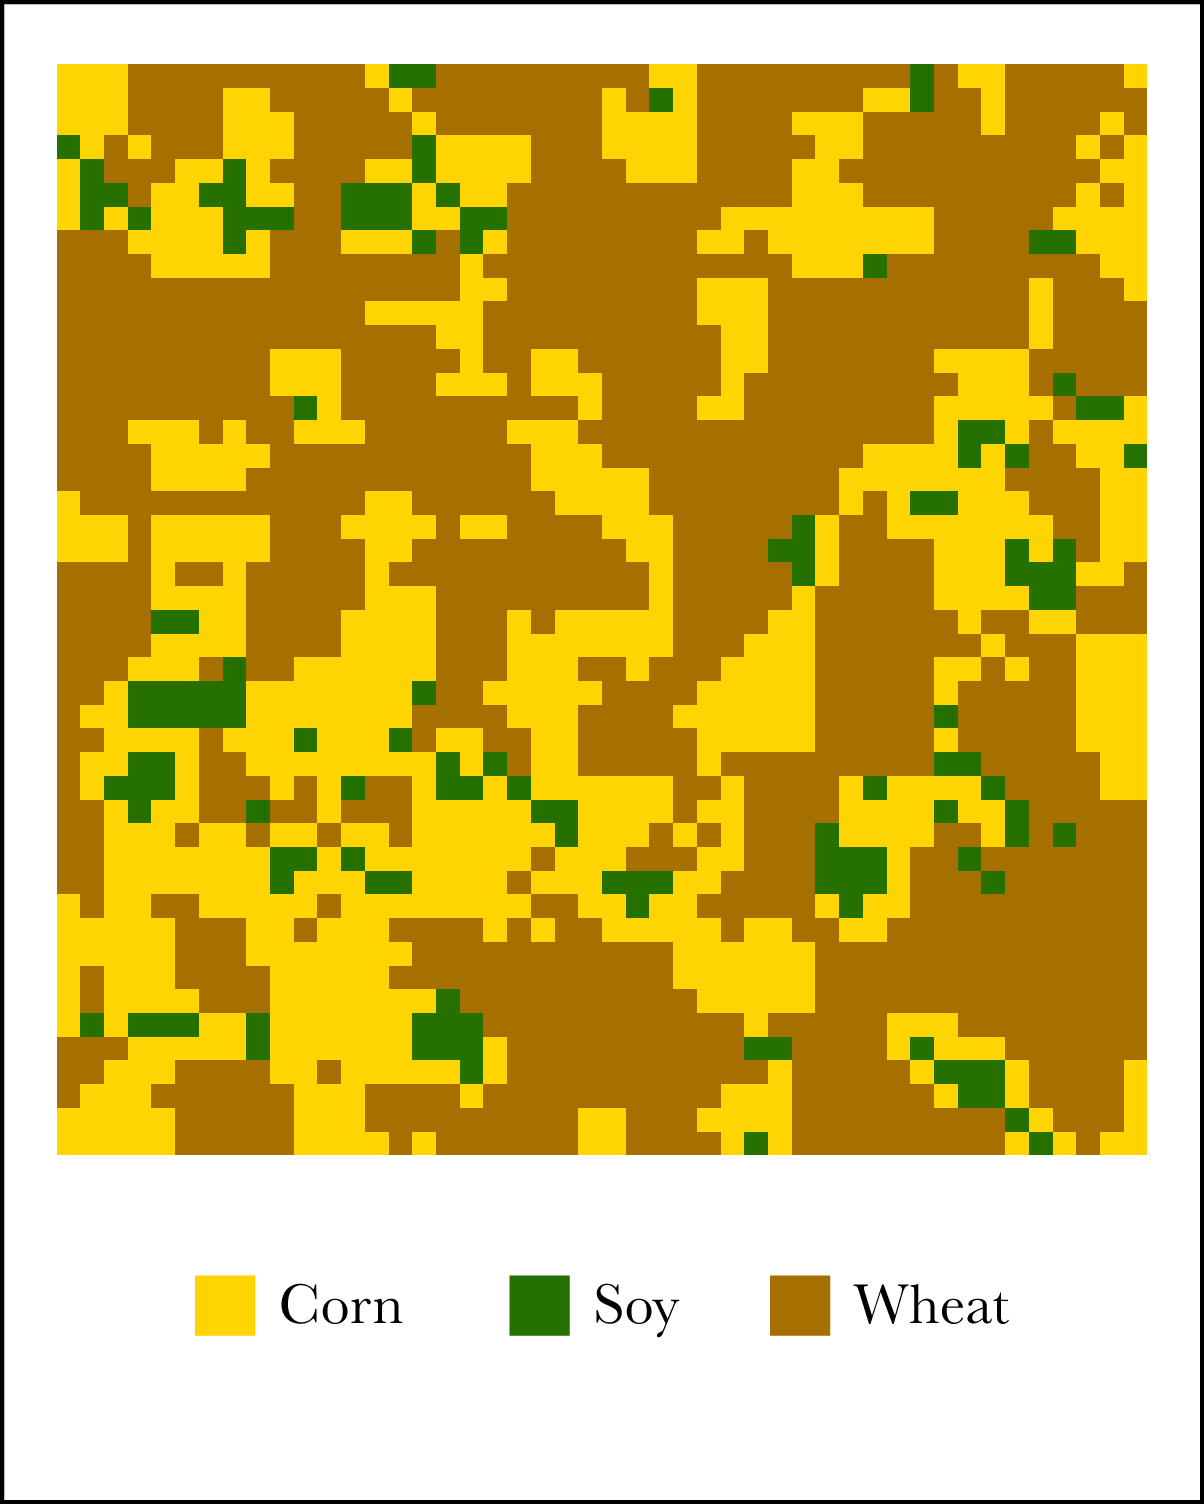
\includegraphics[width=\textwidth]{Graphics/bestfit_edited.png}
    \caption{Best fit image.}
    \label{subfig:bestfit1}
  \end{subfigure}
  \caption{Initial test results.}
  \label{fig:testing1}
\end{figure}


\begin{figure}
  \centering
  \begin{subfigure}[b]{.45\textwidth}
    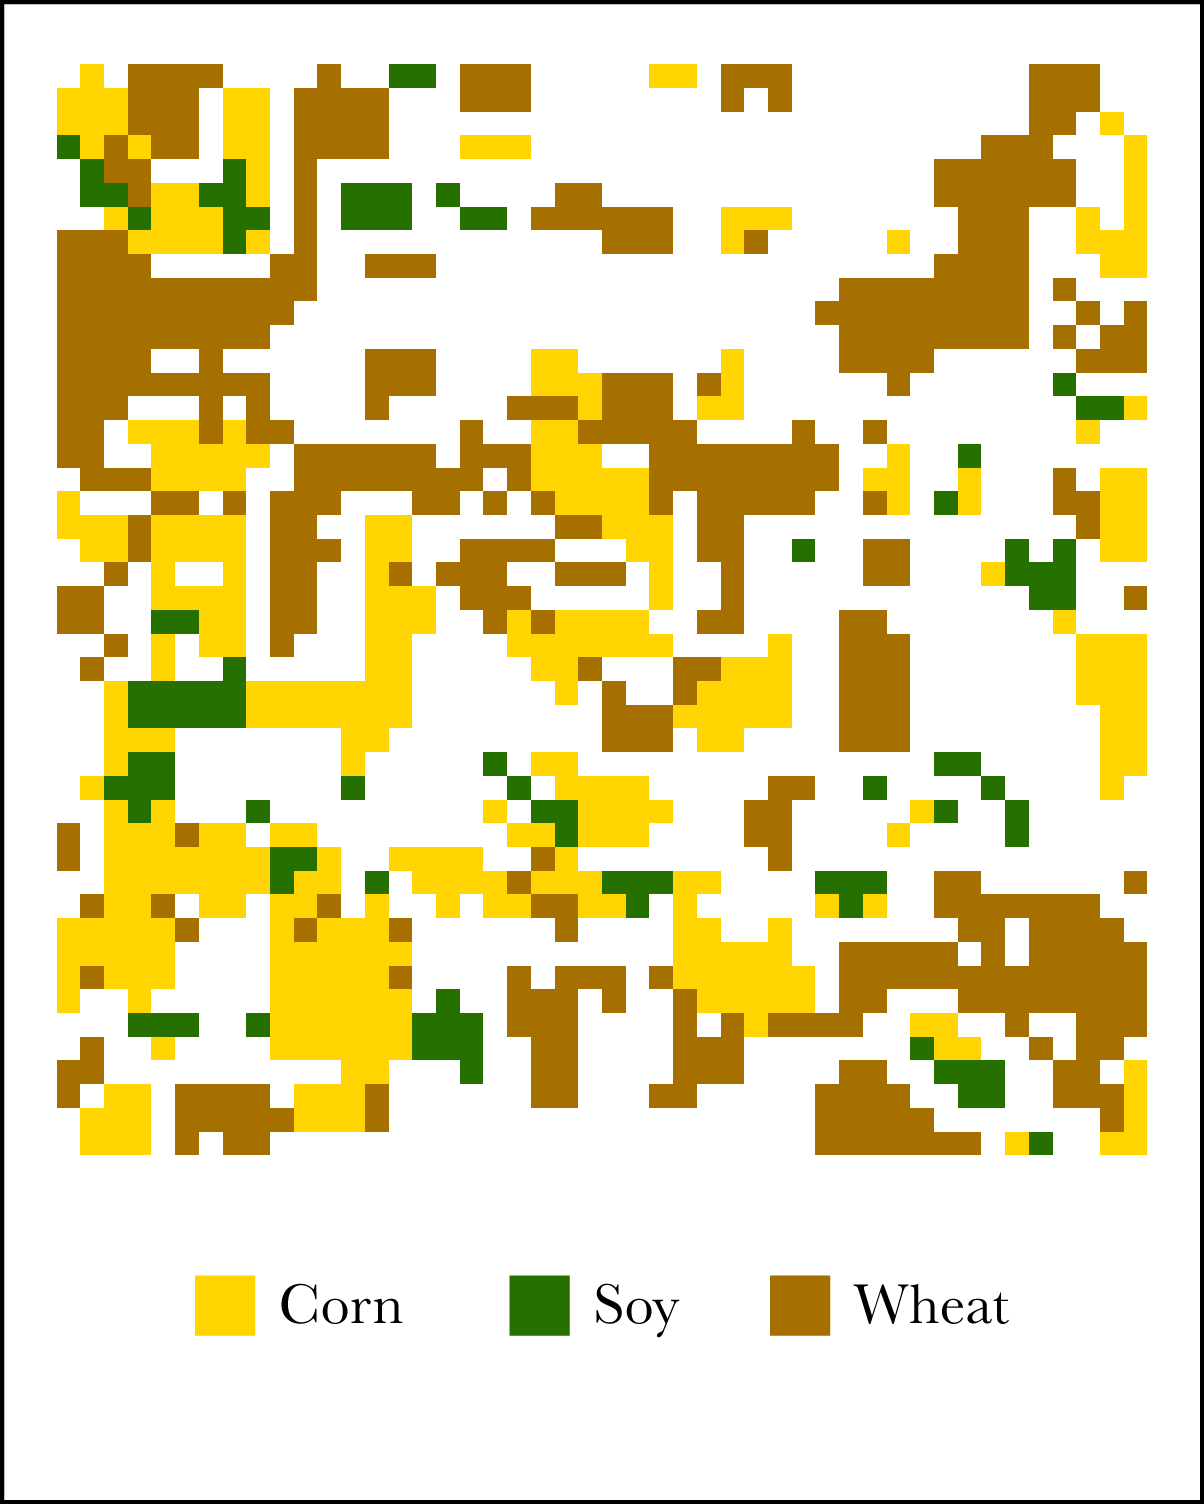
\includegraphics[width=\textwidth]{Graphics/classification1_edited.png}
    \caption{Initial classification of corn, soy, and wheat.}
    \begin{minipage}{.1cm} %fills vertical space to vertical align both subfigures
      \vfill
    \end{minipage}
    \label{subfig:classification1}
  \end{subfigure}
  \quad
  \begin{subfigure}[b]{.45\textwidth}
    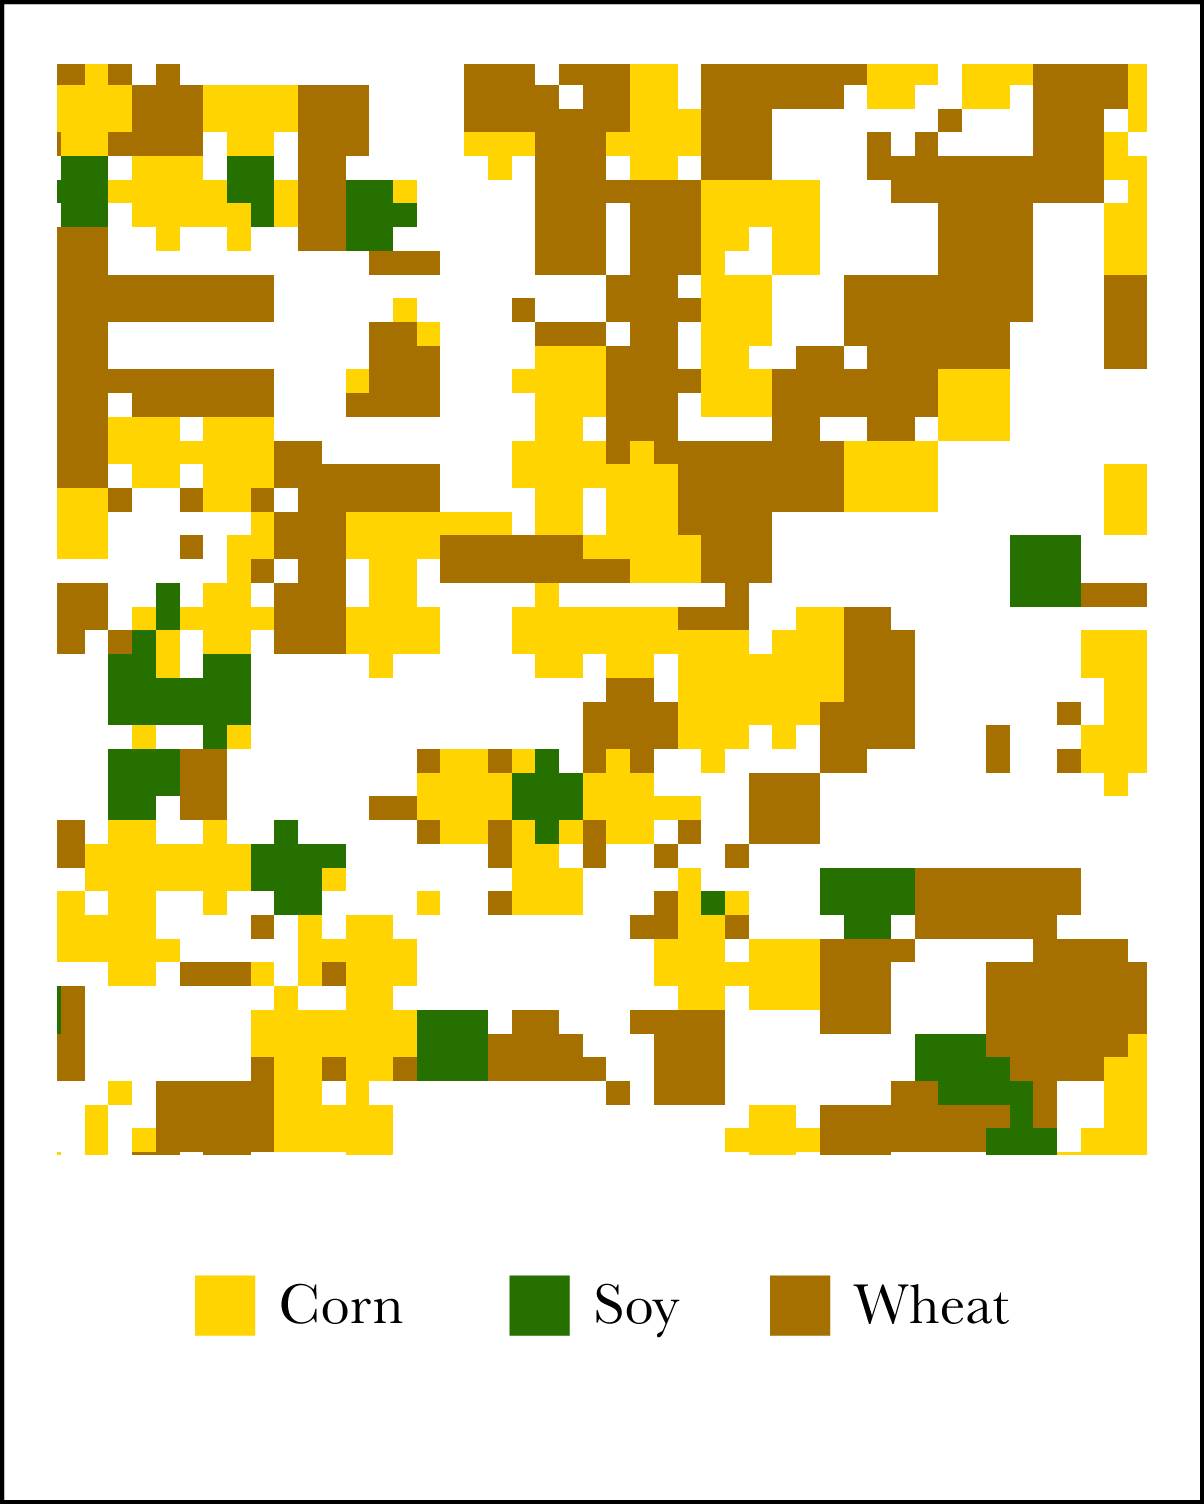
\includegraphics[width=\textwidth]{Graphics/cdl_rsmp_edited.png}
    \caption{2012 USDA CDL, resampled to 250m pixels to match MODIS data.}
    \label{subfig:CDL}
  \end{subfigure}
  \caption{Initial classification and ground truth}
  \label{fig:classification}
\end{figure}


\begin{table}
  \centering
  \caption{Accuracy assessment of the initial results.}
  \label{table:acc}
  \begin{tabular}{rcccccc}
    \toprule
     & Corn & Soy & Wheat & Other & Total & User Accuracy \\
    \midrule
    Corn & 260 & 22 & 6 & 103 & 391 & 67\% \\
    Soy & 10 & 59 & 1 & 29 & 99 & 60\% \\
    Wheat & 33 & 0 & 354 & 127 & 514 & 69\% \\
    Other & 174 & 27 & 241 & 670 & 1112 & 60\% \\
    Total & 477 & 108 & 602 & 929 & 2116 \\
    Producer Accuracy & 55\% & 55\% & 59\% & 72\% \\
     &  &  &  &  &  & Overall: 63\%\\
     &  &  &  &  &  & Kappa: 0.443 \\      
    \bottomrule
  \end{tabular}
\end{table}


\section*{Anticipated Outcomes}

Upon the completion of my research, I expect to have a working tool which can be used as an economical and effective means of crop classification. With the results of my testing, I will know how changes in the generation of the reference curves effects the results of the classifier. Using this tool and knowledge, I will generate crop maps of my study areas, and quantify their accuracies. The results of this study should be of value to those working in the field of remote sensing and those investigating LULC change, particularly in regard to deforestation and agriculture. I hope this work will be the basis for future investigations into soy's role in Argentina's deforestation.


















